\documentclass[output=paper]{langscibook}
\ChapterDOI{10.5281/zenodo.18845938}
\author{Draško Kašćelan\orcid{}\affiliation{University of Essex} and María del Carmen Parafita Couto\orcid{}\affiliation{University of Santiago de Compostela}}
\title[Code-switching by individuals with neurodevelopmental conditions]{Code-switching by individuals with neurodevelopmental conditions: A scoping review}
\abstract{Code-switching or the use of more than one language in an utterance or in conversation is a natural and often quite frequent phenomenon in bilingualism. While there have often been concerns about bilingualism in neurodivergent populations, to date no comprehensive overview has been done on code-switching practices among neurodivergent individuals (children or adults). In this scoping review, we aim to: (i) identify neurodevelopmental conditions in which code-switching has been investigated; (ii) identify approaches used to explore code-switching in this population; (iii) describe the demographic and bilingualism-related characteristics of investigated populations; (iv) outline any comparisons in code-switching practices between neurodivergent and neurotypical bilinguals; (v) outline attitudes towards code-switching in the investigated population. Among the scarcely conducted research on the topic (n = 31 sources), we uncover that code-switching has primarily been explored in individuals with autism and with language disorder. The review identifies underrepresentation in research from most areas outside of North America and Europe, as well as underrepresentation in research with older children and adults. We discuss the plethora of methodological approaches used to explore code-switching in neurodivergent populations and their ecological validity. The characteristics of code-switching in neurodivergent individuals are also addressed, as well as the implications of these findings for educators, speech and language therapists, researchers, and bilingual families with neurodivergent family members.}
\IfFileExists{../localcommands.tex}{
  \addbibresource{../localbibliography.bib}
  \usepackage{tabularx,multicol}
\usepackage{url}
\urlstyle{same}

 
\usepackage{langsci-optional}
\usepackage{langsci-lgr}
\usepackage{langsci-gb4e}

\usepackage{multirow}
\usepackage{cleveref}
\usepackage{subfigure}
\usepackage{langsci-branding}

  \input{../localcommands} 
  \input{../localhyphenation} 
  \togglepaper[8]%%chapternumber
}{}

\begin{document}
\maketitle 
%\shorttitlerunninghead{}%%use this for an abridged title in the page headers

\section{Introduction}

In recent years, research on bilingualism in various neurodevelopmental conditions has been expanding.\footnote{We note that the introduction and the methods sections of this chapter are expanded and adapted versions of the content written up for the pre-registered protocol of this scoping review (see \citealt{KascelanParafitaCouto2022}).} This has been particularly observed in conditions such as autism and Developmental Language Disorder (DLD). A large portion of this work has been motivated by parental or practitioner concerns regarding bilingual development in this population (e.g.,  \citealt{Kay-RainingBirdEtAl2012}). Specifically, does acquiring more than one language pose challenges for neurodivergent children? In light of this question, several reviews of the literature have emerged indicating no detrimental effects of bilingualism\footnote{In this paper we often use the terms bilingual(ism) and multilingual(ism) interchangeably.} either across neurodevelopmental conditions \citep{UljarevićEtAl2016} or in some conditions such as autism (\citealt{PrévostTuller2021}). Nevertheless, a variety of methodological confounds and unexplored areas, as noted in \citet{PrévostTuller2021}, might prevent us from generalising these findings across the population.
One aspect of bilingualism which has not been addressed in existing reviews of bilingualism and neurodevelopmental conditions is code-switching. Code-switching or the use of more than one language in an utterance or in conversation is a natural and often quite frequent phenomenon in bilingualism. Taking a clause as a unit of analysis, code-switching can include:

\ea
  \ea \label{ex1a} A switch within a clause (intra-clausal switching); a Welsh-English example taken from the Siarad corpus, Stammers6, line 6 \citep{DeucharEtAl2014}\\
      \gll Mae      yn    lle    lovely\\
      be.3\textsc{sg}.\textsc{pres}  in  where  lovely\\
      \glt ‘It’s a lovely place’
  \ex \label{ex1b} A switch between clauses (inter-clausal switching); a Spanish-English example taken from the Miami corpus, Herring12, line 165 \citep{DeucharEtAl2014}\\
      \gll Quiero      ir        quiero      ir   but    like    I      don’t   wanna             go     by    myself\\
      want.1S.\textsc{pres}    go.INF      want.1S.\textsc{pres}   go.INF but  like  I.1S  do.1S.\textsc{pres}+NEG want.INF+TO  go.INF  by    myself.1S\\
      \glt ‘I want to go, I want to go but, like, I don’t wanna go by myself’
  \z
\z

Apart from its prevalence, work on code-switching in neurotypical populations has indicated that code-switching gives a unique insight into the nature of one’s linguistic competence (\citealt{Poplack1980,QuinYowEtAl2018,TruscottSharwoodSmith2017}), language representation (\citealt{TruscottSharwoodSmith2017}), and potential cognitive mechanisms of bilingual language control (\citealt{Hofweber2019}). Furthermore, code-switching is an important indicator of linguistic community norms (\citealt{Deuchar2020,ParafitaBalamnodate}) which need to be acquired for speakers to be fully functioning members of a specific group (\citealt{PhillipsDeuchar2021}). Taking into account the importance of code-switching for understanding bilingual development and lived experiences of bilinguals, it is vital to identify to what extent code-switching has been explored in neurodivergent individuals. Furthermore, considering the role that code-switching plays in the formation of bilingual identities (e.g.,  \citealt{MyersScotton1983, YimClément2021}) as well as the importance of maintaining bilingualism for child wellbeing \citep{MullerEtAl2020}, it is necessary to offer state-of-the-art guidance for practitioners (such as educators and speech and language therapists) in terms of advice on code-switching to be provided to bilingual families with neurodivergent family members.

To address this, we aim to conduct a scoping review of code-switching in bilinguals with various neurodevelopmental conditions. There are several reasons for opting to use the scoping review methodology to achieve this aim rather than rely on alternative forms of evidence synthesis. Specifically, scoping reviews are best suited to explore the breadth of research -- that is, they show what evidence exists rather than what is effective \citep{MunnEtAl2022}. Furthermore, they are ideally suited for mapping out and summarising the available evidence, identifying gaps in research/knowledge, and informing future research or systematic reviews with more specific research questions (\citealt{PetersEtAl2021updated, TriccoEtAl2018}). Scoping reviews can also include work implementing quantitative, qualitative, or mixed methods, as well as various sources of evidence -- published academic research, unpublished work, other reviews, or non-academic documents, such as policy documents or online media (\citealt{PetersEtAl2021scoping}). In line with the aims of the scoping review methodology, we are casting our search net wide in order to identify any research on code-switching in individuals with neurodevelopmental conditions. As will be discussed further below, this will lead to the use of terminology and identification of related but different language mixing phenomena that do not necessarily correspond to the definition of code-switching which we provided in examples \REF{ex1a} and \REF{ex1b} above. These differences and their implications are highlighted in the discussion section.

In the following section we outline five research objectives of this scoping review addressed through ten research questions. In the methodology section, the procedure implemented for conducting this scoping review is comprehensively described. This is followed by the presentation of the results and the discussion of findings with implications for the life outcomes of neurodivergent bilinguals, as well as for educational, and speech and language therapy practice.

\section{Objectives}

This scoping review aims to map the available evidence on code-switching in bilinguals with neurodevelopmental conditions across bilingual contexts in order to: (i) identify neurodevelopmental conditions in which code-switching phenomena have (not) been investigated; (ii) identify approaches used to explore code-switching in this population; (iii) describe the demographic and bilingualism-related characteristics of investigated populations; (iv) outline any comparisons in code-switching practices between neurodivergent and neurotypical bilinguals; (v) get a sense of attitudes towards code-switching and advice given regarding code-switching in the investigated population. The following research questions will be addressed:

\begin{enumerate}
  \item In which neurodevelopmental conditions has code-switching been investigated? \textit{[objective (i)]}
  \item Was code-switching the main focus of investigation or addressed sporadically? \textit{[objective (ii)]}
  \item Which method was used to analyse the code-switching data: quantitative, qualitative, mixed methods? \textit{[objective (ii)]}
  \item Which approach was used to explore code-switching in this population: spontaneous speech, semi-experimental approach, experimental approach, a combination? \textit{[objective (ii)]}
  \item What was the number of participants in studies investigating code-switching in neurodivergent bilinguals? \textit{[objective (iii)]}
  \item What were the demographic characteristics of communities in which code-switching has been investigated (geographic location, language combinations, age range of participants, participants’ sex and gender distribution, socioeconomic status)? \textit{[objective (iii)]}
  \item Have studies of code-switching in neurodivergent individuals included a neurotypical bilingual comparison group? \textit{[objective (iv)]}
  \item Are there any indications that code-switching happens differently in neurodivergent individuals in comparison to neurotypical ones? \textit{[objective (iv)]}
  \item What kind of professional advice have respective individuals received regarding code-switching: positive, negative, both, neither, no data? \textit{[objective (v)]}
  \item How is code-switching perceived in the environment of neurodivergent individuals: positively, negatively, both, neither, no data? \textit{[objective (v)]}
\end{enumerate}

\section{Methods}

\subsection{Protocol and pre-registration}

A scoping review protocol was prepared and registered prior to conducting the review in accordance with the Joanna Briggs Institute (JBI) methodology for scoping reviews and informed by the guidance provided in \citet{PetersEtAl2022} and \citet{PollockEtAl2022}. The registration of the protocol was conducted on the Open Science Framework (OSF) on 17  {August 2022} (\url{https://osf.io/ru8pe}). Throughout the chapter, we specify in footnotes whether there were any departures from the pre-registered protocol and clarify the rationale for those decisions. At the time of pre-registering the protocol, we did not identify any previous or ongoing reviews on the topic in The International Prospective Register of Systematic Reviews (PROSPERO) database. The PROSPERO database has also been checked recently, and we identified a protocol for a systematic review on code-switching by \citet{SnijdersEtAl2023} registered on 03  {December 2023}. However, as the registered systematic review protocol by \citet{SnijdersEtAl2023} focuses on code-switching in neurotypical children between the ages of 2 and 6 years, it does not address the aims proposed in this scoping review.

\subsection{Eligibility criteria and information sources}

We strictly adhered to the decisions on eligibility criteria and information sources as reported in the pre-registered protocol (\citealt{KascelanParafitaCouto2022}). The table and the text in this section are close adaptations from the protocol. \tabref{tab:kascelan:1} reports the eligibility criteria for inclusion through a summary of the population, the concept, and the context of interest.

\begin{table}
\begin{tabularx}{\textwidth}{lQ}
\lsptoprule
PCC Element & Specification\\
\midrule
Population & { We focused on bilingual individuals (of any age, gender, sex, socioeconomic status) with any neurodevelopmental conditions as defined by the Diagnostic and Statistical Manual of Mental Disorders, Fifth Edition (DSM-5;  \citealt{AmericanPsychiatricAssociation2013}) with a few additions of terms of our own as explained in the search strategy below. We included papers even if they simply stated that participants had a particular diagnosis, without a need for a formal confirmation of how the diagnosis had been made. Research with participants with more than one condition was also included.} \\
Concept & { The concept under investigation is code-switching. In this review, we use \textit{code-switching} as an overarching term for any language-mixing practices (i.e., use of more than one language in an utterance or in conversation). All types of code-switching were eligible for inclusion. See the search strategy below for the specification of code-switching types and terms which we used when searching the literature.} \\
Context & { The scoping review focuses on any bilingual/multilingual communities with no restrictions regarding the geographic location or the nature of bilingualism (e.g., simultaneous, sequential, etc.).  See the search strategy below for the specification of bilingualism-related terms which were used when searching the literature.} \\
\lspbottomrule
\end{tabularx}
\caption{Specification of the Population, Concept, Context (PCC) of the scoping review.}
\label{tab:kascelan:1}
\end{table}

There were no restrictions for inclusion in terms of methodology as we aimed to include quantitative, qualitative, and mixed methods studies. Furthermore, any approach to investigating code-switching was included: work with spontaneous speech, semi-experimental approach, experimental approach, a combination of these.

The scoping review includes published articles, chapters, books, and conference proceedings, as well as unpublished and grey literature, such as preprints and dissertations. As indicated in \citet{KascelanParafitaCouto2022}, work excluded at the stage of full text screening can be found via a link provided in supplementary materials, which leads to an OSF page containing a complete dataset and the exclusion reasons specified.

Whenever we identified any sort of evidence synthesis on this topic, rather than including it in the review, we followed up on the original papers reviewed in the identified synthesis. Nevertheless, the identified synthesis papers are still acknowledged in our dataset (see supplementary materials) as sources of evidence.

Identification of resources was conducted through the search of databases and through alternative ways of identifying relevant work. The following electronic databases were used as a source of information: Ovid (Embase Classic+Embase, Global Health, APA PsycInfo), ProQuest, Scopus, and Web of Science.\footnote{During the time of this scoping review’s protocol drafting, the first author was affiliated with the University of Leeds. Consequently, the University of Leeds library resources were used to select these databases for the final search. These databases were listed as popular for research in health, medicine, psychology, arts, social sciences, and related subjects.} The databases were searched on 13  {March 2023}. It was decided not to have date restrictions for any database, as we aimed to include any relevant work in our review. The start and the end date varied across databases due to the scope of time that each database has. The project's OSF page (\url{https://osf.io/4nwgd/}) contains an example report of a search conducted in one of the databases and it illustrates the date restrictions imposed by the database scope (e.g., for APA PsychInfo, this was from 1806 to February Week 4 2023).

In addition to the database search, there were three alternative ways of identifying relevant work. First, prior to conducting the database search, we identified some relevant work through our knowledge of and interaction with the literature on bilingualism and neurodevelopmental conditions. Second, in order to obtain published and unpublished work which might not be picked up in the database search, we sent a notice about the scoping review (see a draft notice in the protocol Appendix) via several mailing lists and networks (ISB\_list, Info-CHILDES, Bi-SLI COST Action, The LINGUIST List) and on social media (Twitter, Facebook). In this notice, we asked colleagues to send us any (un)published work on code-switching in bilinguals with neurodevelopmental conditions if they would like for it to be included in the review. These notices were sent out in  {March 2023}. Third, after the database search was conducted and throughout the screening process, we monitored relevant literature and included any work which has not already been identified -- this work did not go through the abstract screening stage; rather these papers were fully screened. The routes of information sources are summarised in \figref{fig:kascelan:1}, in the identification section.

There were no language restrictions in our search. However, texts in languages not spoken/understood by the authors were excluded. Information on this can be found in the dataset on the project's OSF page (\url{https://osf.io/4nwgd}).

\subsection{Search and selection of sources of evidence}

The complete list of key terms used for the search in electronic databases can be found in \tabref{tab:kascelan:2} of the pre-registered protocol (\citealt{KascelanParafitaCouto2022}). There were three sets of key terms:
(1) Key Term 1 was participant-related (e.g., neurodevelopmental disorder*, autism spectrum condition*, DLD, vocal tic disorder*, etc.),
(2) Key Term 2 was concept-related (e.g., code-switch*, alternation*, intra-clausal*, borrow*, translanguag*, etc.), and
(3) Key Term 3 was context-related (e.g., bilingual*, BFLA, L2, societal language*, etc.). The list of terms was finalised during several discussions between the two authors. For the purposes of this review, we use the term code-switching interchangeably with terms such as language mixing or code mixing. Specifically, due to the nature of scoping reviews (which require casting the search net as wide as possible), for the Key Term 2 (concept-related), we use various code-switching terminology which does not necessarily refer to the same phenomena (e.g., inter-clausal, inter-sentential, insertions, translanguaging, language mixing, code-switching, code mixing, etc.). However, we acknowledge the lack of consensus in the field in terms of differentiating between code-switching, language mixing, or code-mixing (see for example \citealt{GullbergEtAl2009} for a discussion) as well as different assumptions underlying code-switching and translanguaging (\citealt{Balam2021, Li2018}). We return to this point in the discussion of the review findings.

When searching the electronic databases, each term within the category \textit{Key Term 1} was linked with a boolean operator \textit{OR}. The same was done for terms within the categories \textit{Key Term 2} and \textit{Key Term 3}. Following this, the key terms were connected with a boolean operator \textit{AND}, as follows: (\textit{Key Term 1) AND (Key Term 2) AND (Key Term 3)}. The search strategy was adapted for each included database. An example report of a search conducted in one of the databases can be found on the project's OSF page, including necessary filters and search syntax adaptations: \url{https://osf.io/4nwgd/}. The first author conducted the search in all databases following the university library resources for conducting reviews.

The selection of resources is visually represented in \figref{fig:kascelan:1}. We collected 273 resources (i) through the identification of resources by the authors prior to the database search, (ii) through the search of four databases, and (iii) through communication with colleagues in the field. These were exported to an excel file (see the \textit{inclusion-exclusion sheet} in the dataset on the project's OSF page). Following this, 121 duplicates were identified and removed. The remaining 152 abstracts were screened independently by both authors and the following exclusion criteria were applied:
(1) not available,
(2) not in a language that reviewers speak/understand,
(3) not about bi/tri/multilingualism,
(4) not about code-switching,
(5) not about neurodevelopmental conditions, or
(6) other (specification required). Independent abstract screening resulted in disagreement regarding 13 out of 152 abstracts (i.e., in only 8.6\% of cases). The authors discussed the disagreements until a consensus was reached.

This left us with 34 papers for full text screening. A randomly selected subset of these (approximately a third: 11/34 or 32.4\%) was independently screened fully by both authors.\footnote{This was one of the rare cases in which we departed from the pre-registered protocol. According to the protocol, we intended to independently complete full text screening of all the resources. However, due to personal circumstances of the second author and time restrictions, the second author fully screened a randomly selected subset (i.e., approximately a third of the dataset).}  The authors disagreed in 4 out of 11 cases (i.e., in 36.4\% of cases). Considering the large exclusion/inclusion disagreement rate in full text screening, the authors had an extensive discussion until consensus was reached. Following that discussion, the first author fully screened the rest of the data, consulting the second author whenever in doubt. This left us with 14 papers for inclusion in the review.

Following this, the reference lists of the 34 papers that were fully screened were also checked for any relevant literature.\footnote{This is another departure from the pre-registered protocol. Specifically, according to the protocol, we aimed to screen the references only in the papers included in the review after the full text screening, which in this case would be 14 papers. However, to avoid missing relevant work, we screened the references of all 34 papers that were fully screened.} This led us to identify 25 references which could potentially be included in the review. The full text screening of these 25 papers was completed by the first author in consultation with the second author whenever in doubt. This resulted in: excluding 1 resource due to its inaccessibility, excluding 18 resources for additional reasons as per the previously outlined exclusion criteria, and keeping 6 resources in the review. The lists of these 25 papers identified in references with reasons for exclusion and additional notes can be found in the \textit{identified in references} sheet in the datafile on the project's OSF page.

\begin{figure}
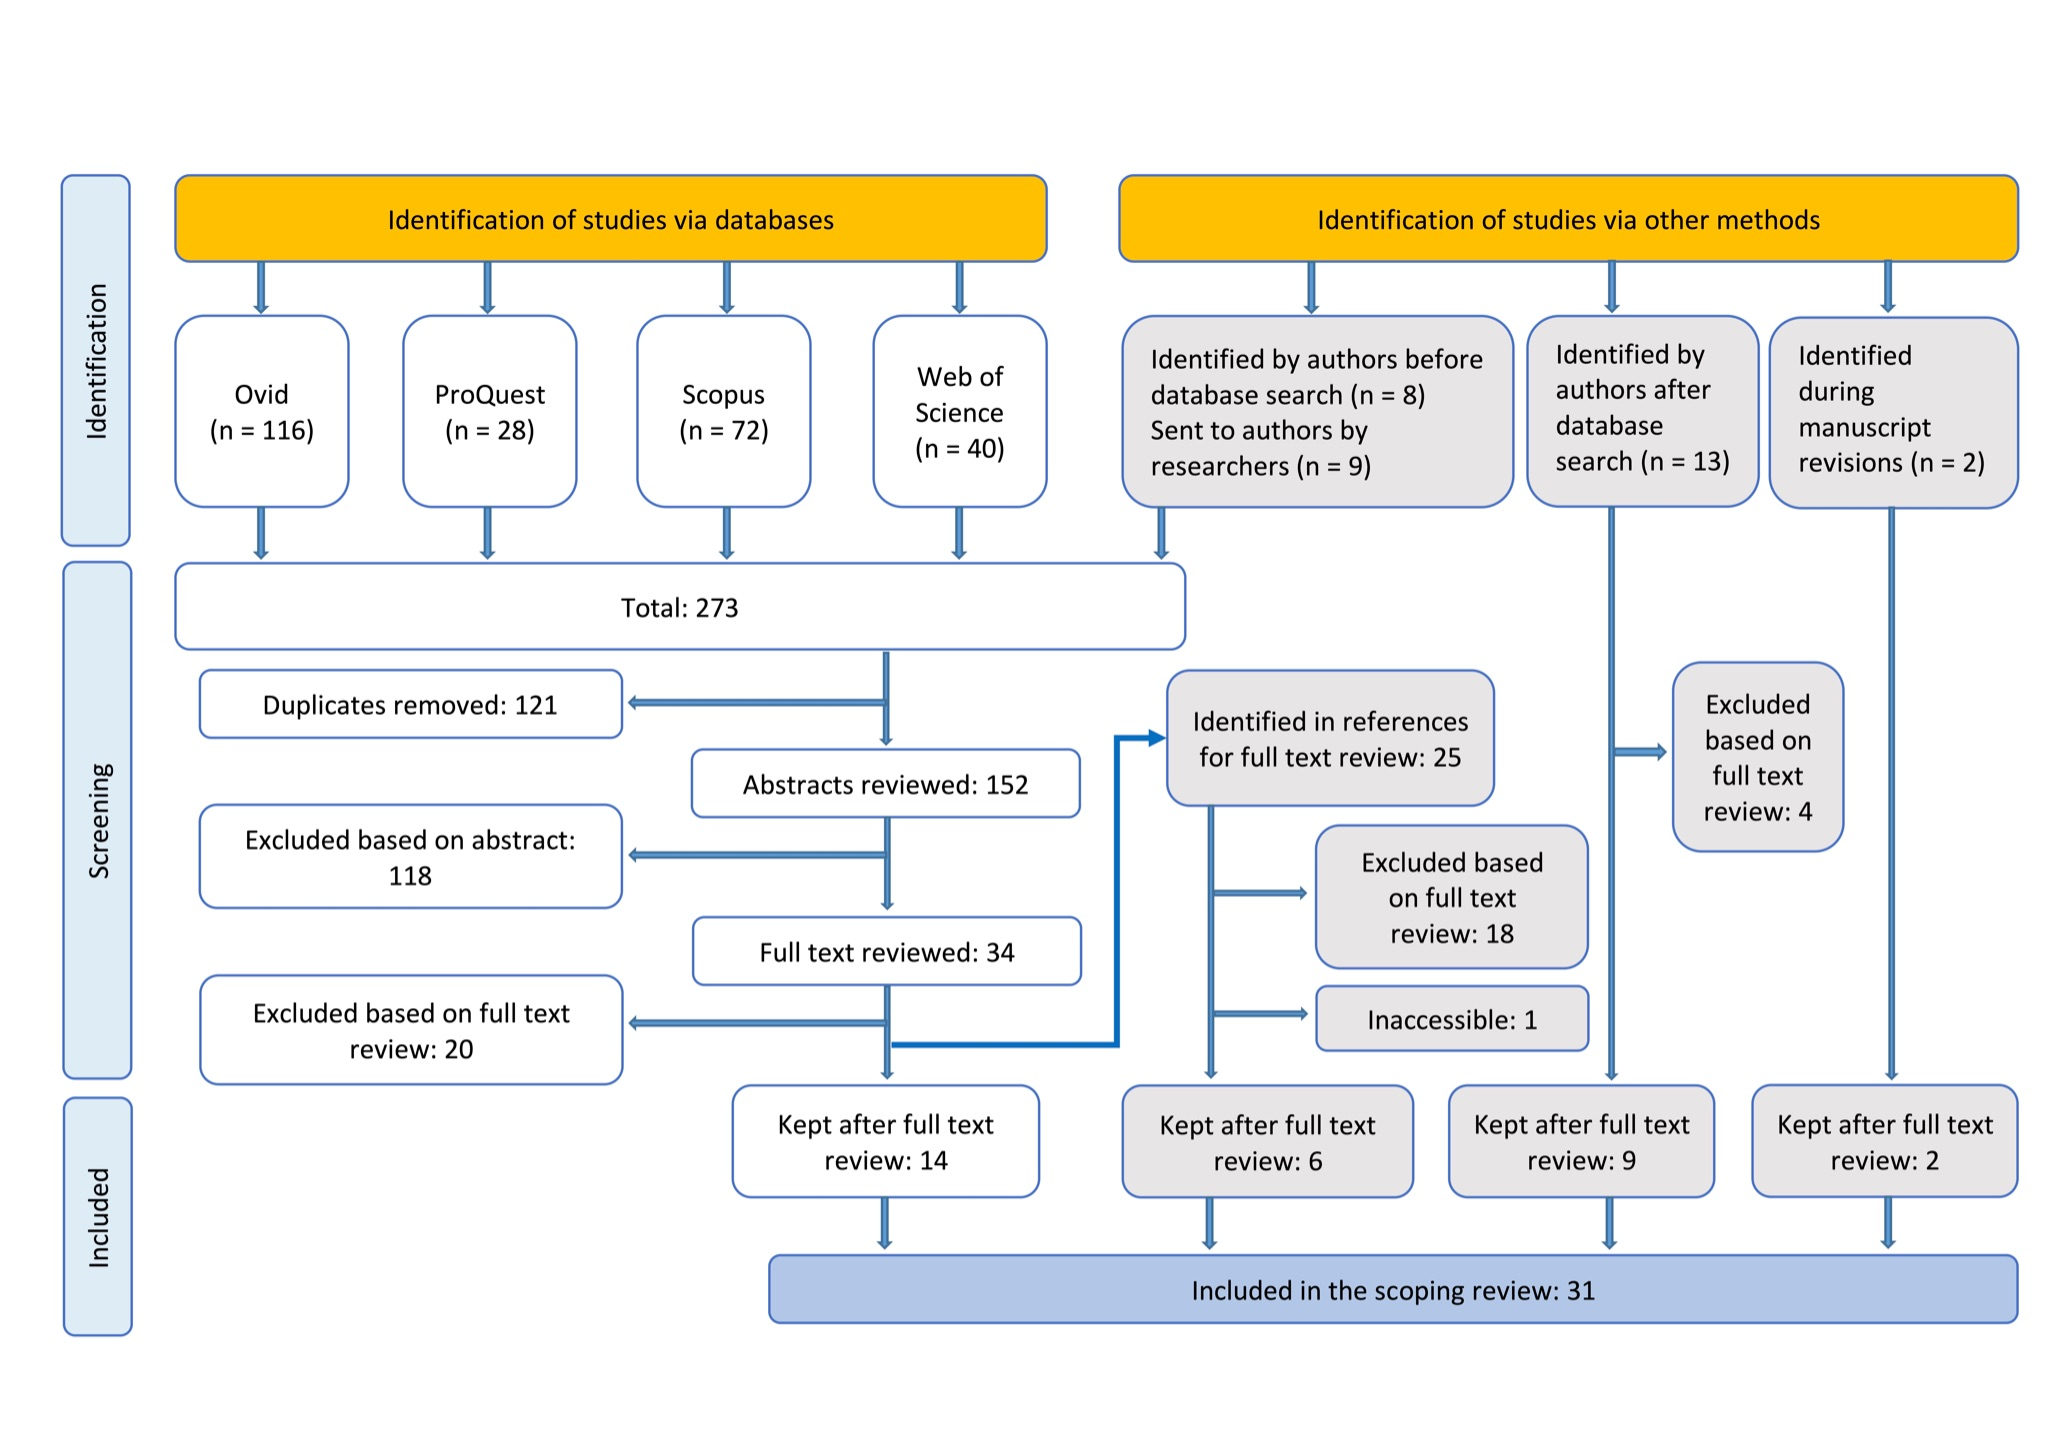
\includegraphics[width=\textwidth]{figures/KaelanandParafitaCouto-img001.jpg}
\caption{The Preferred Reporting Items for Systematic Reviews and Meta-Analyses (PRISMA) flowchart of the scoping review process.}
\label{fig:kascelan:1}
\end{figure}

While we were screening the resources identified in the databases and gathered through the above-outlined alternative approaches, we also monitored relevant literature for any new research published after our database search or for any research that we potentially missed. Over the period of about 9 months, we identified 13 potential resources, which were fully screened by the first author in consultation with the second author when required. Of these, 4 resources were excluded and 9 were kept for inclusion in the scoping review. The details about these papers, the exclusion reasons and relevant notes can be found in the \textit{identified after review} sheet in the datafile on the project's OSF page.

Finally, during this chapter’s revision process, we were sent a recently published paper on the topic by the paper's authors \citep{BlomEtAl2024} to consider for inclusion in the scoping review. In addition, in \citegen{BlomEtAl2024}  references, we identified another relevant paper for inclusion (\citealt{GrossCastilla-Earls2023}). Both of these papers were included in the scoping review (the details about these papers can be found in the \textit{identified during revisions} sheet in the datafile on the project's OSF page). Since they were both published after our database search (i.e., after 13  {March 2023}), it is clear why they were not picked up via the key term search.

Following this procedure, we were left with 31 papers for data extraction and analysis. Of these 31 papers, 27 were published / accepted for publication (22 journal articles, 4 book chapters, 1 proceeding) and 4 were unpublished dissertations.\footnote{As pointed out by an anonymous reviewer, a part of the dissertation by  \citet{AnguloJimenez2020} has recently been published as a journal article (\citealt{Angulo-JimenezDeThorne2024}). Consequently, we acknowledge this publication here and in the reference list.} The above-outlined process is visually represented in \figref{fig:kascelan:1}.

\subsection{Data charting process and data items}

A data charting form was developed jointly by both authors. The developed version was posted on the project's OSF page with the pre-registered protocol on 17  {August 2022} (sheet \textit{data extraction sheet}). Of the 31 resources for data extraction, 3 were randomly selected (\citealt{Gutiérrez-ClellenEtAl2009, Iluz-CohenWalters2012, SoesmanEtAl2022}) and their data was independently extracted by both authors in the existing data charting form. Following this, the authors met to discuss the adequacy of the data charting form and made minor changes. A column titled \textit{Gender or Sex explicitly labelled in the paper} was added for specification when resources did not distinguish between sex and gender and when we had to assume which one they referred to in their descriptive statistics. The column \textit{Group differences in code-switching (y/n)} was renamed to \textit{Group differences/characteristics of code-switching} to allow the extraction of data when a comparison group was not included but rather only the description of code-switching practices of neurodivergent individuals were available. The column \textit{Group differences in code-switching code} was added to allow for a coding of whether the groups (when present) differ in their code-switching practices and to what extent: no, both (predominantly no), both, both (predominantly yes), yes, inconclusive, or not applicable (na). We also added a column \textit{Comments} for any additional points or notes that might facilitate data analysis. Following this data charting form calibration, the first author extracted the data from the rest of the resources. Once this step was completed, the authors met to discuss the data and resolve any difficulties in data extraction or classification, particularly in relation to the decisions on the degree of differences in code-switching identified between neurodivergent and neurotypical individuals or the lack of equivalency in data on participants’ socioeconomic status. Throughout the data extraction and analysis process, a few other columns were added to the data extraction sheet as agreed by both authors. The datafile (sheet \textit{data extraction sheet}) contains a note on these columns indicating that they were added after the protocol registration. The complete datafile can be accessed on the project's OSF page (see Supplementary materials for the link to the OSF page).

We extracted the data on the following variables: resource description (document number, author(s), publication year, title, document type), objective I (neurodevelopmental condition(s) investigated), objective II (whether code-switching was the main focus of investigation, the method used to explore code-switching, and the approach used to investigate code-switching), objective III (number of neurodivergent participants, geographic location of the studies, language combinations, participant age range, participant sex and gender distribution, participant socioeconomic status), objective IV (inclusion of the neurotypical comparison group, group differences/characteristics of code-switching), and objective V (professional advice on code-switching and perception of code-switching in the environment of neurodivergent individuals).

\subsection{Critical appraisal and synthesis of results}

Our research objectives did not include explicit critical appraisal of each study included in the review. Consequently, such appraisal was not explicitly conducted. However, in the results and the discussion sections, the analysis of the extracted data will include the quality assessment of gathered evidence. In particular, we will address the contributions and limitations of existing research as well as its implications for future research and the effects that existing approaches might have on the life outcomes of the target community members, educational and speech and language therapy practice.

The resource identification, screening, eligibility, and inclusion are outlined in \figref{fig:kascelan:1}. The datafile on the project's OSF page includes a list of all the studies that went through the outlined process and reasons for exclusion with additional notes where relevant. In the sections below, we will use a combination of tables, figures and narrative to present the data and address all five objectives of the scoping review.

\section{Results}

\subsection{Scope of investigations and focus}

Despite the long list of neurodevelopmental conditions considered in this review, code-switching has been investigated in only a limited number of conditions as indicated in \tabref{tab:kascelan:2}. Specifically, language disorder and autism seem to be predominantly examined in relation to language mixing, while other neurodevelopmental conditions tend to appear sporadically or often as secondary conditions in the investigated samples.

Among the 31 studies, code-switching was the main focus in 18 of them (58\%). It is important to note that out of 13 studies which explored code-switching sporadically, only 1 was identified via the database search, which is expected as the key terms targeted the studies focusing on all aspects of PCC (see \tabref{tab:kascelan:1} above). Of the remaining 12 studies, 4 were identified in references of screened papers, and 8 were identified after the database search. All of these 8 studies were picked up due to the first author’s familiarity with the literature on autism and bilingualism. Consequently, this approach inflated the number of studies focusing on autism indicated in \tabref{tab:kascelan:2}.\footnote{The percentages in the table do not add up to 100\% as some studies had participants with more than one condition. In this table, the term language disorder includes terms such as language impairment, specific language impairment, developmental language disorder, primary language impairment. The term autism includes terms such as autistic disorders, high functioning autism, pervasive developmental disorder, pervasive developmental disorder – not otherwise specified, Asperger’s syndrome, autism spectrum disorder.} However, even if these studies were excluded, autism would still represent a commonly investigated condition in the corpus that was identified.

\begin{table}
\begin{tabularx}{\textwidth}{lYY}
\lsptoprule
Neurodevelopmental condition & Number of studies & \% of studies\\
\midrule
Language disorder             & 16&52\%\\
Autism                        & 14&45\%\\
ADHD                          & 1 & 3\%\\
Down Syndrome                 & 1 & 3\%\\
Non-verbal learning disorder  & 1 & 3\%\\
Prader-Willi Syndrome         & 1 & 3\%\\
Repaired cleft palate         & 1 & 3\%\\
Stuttering                    & 1 & 3\%\\
\lspbottomrule
\end{tabularx}
\caption{Frequency of explored neurodevelopmental conditions.} 
\label{tab:kascelan:2}
\end{table}

\subsection{Methods and approaches to code-switching}

The quantitative method was used predominantly across the studies (n = 20), followed by the qualitative methods (n = 10), while the mixed methods were used only in one study (\citealt{AnguloJimenez2020}). A series of approaches taken to explore code-switching can be broadly grouped as follows: spontaneous speech (n = 6), semi-experimental (n = 5), experimental (n = 6), a combination of these (n = 4), not applicable (n = 10). The studies implementing the spontaneous speech approach included guided conversations with obligatory questions about family, school, games (\citealt{Sanz-TorrentEtAl2007}), mundane naturalistic conversations (\citealt{AnguloJimenez2020,Yu2013}), typical daily interactions \citep{CohenEtAl2025}, interactions with a therapist \citep{Ponce-Lawler2017}, and a written diary \citep{Karniol1992}. Studies with semi-experimental designs relied on story retellings (\citealt{Aguilar-MediavillaEtAl2024,KapantzoglouEtAl2021}), narrative elicitation \citep{Mammolito2015}, or narrative elicitations and story retellings (\citealt{GrossCastilla-Earls2023,Iluz-CohenWalters2012}). The experimental studies included a range of tasks: cued picture selection (\citealt{KingEtAl2021}), cued picture naming \citep{SnijdersEtAl2025}, sentence repetition \citep{SoesmanEtAl2022}, acceptability judgement and sentence completion (\citealt{LicerasGarcia-Alcaraz2019}), repeated word association \citep{ShengEtAl2012}, and expressive language assessments \citep{Pert2007}. The four studies which combined these approaches included an experimental and a semi-experimental task (guessing and description phases of a scripted confederate dialogue task, \citealt{GrossKaushanskaya2022}), or semi-experimental tasks (narrative/story retell and/or elicitation) and a spontaneous conversation (\citealt{BlomEtAl2024, Gutiérrez-ClellenEtAl2009, Restrepo2003}). Ten studies did not include any particular approach to code-switching as these were among the studies in which code-switching was not the main focus of research. We return to the implications of using various approaches to examining code-switching in the discussion section.

\subsection{Number of neurodivergent bilinguals and demographics}

Across 31 identified papers, there were in total 373 neurodivergent (range: 1-49) and 401 neurotypical (range: 3-65) participants. The 31 papers included 32 studies in total. Focusing on the neurodivergent participants only, about a third of the studies (n = 11) could be classified as case studies (1-3 participants), while 13 studies had between 4 and 20 participants. Only 6 studies included data about more than 20 participants (range: 23-49). Finally, 2 studies included research with practitioners as participants rather than neurodivergent individuals.

In terms of geographic distribution reported in the identified 31 papers, the neurodivergent participants resided predominantly in the USA (n = 17 studies), across various parts of the country (as specified in some of the studies): a midwestern city, a metropolitan area in north-western USA, southern California, metro Atlanta area, El Pueblo -- Midwest, El Paso -- Texas, Greater San Francisco Bay area, Austin -- Texas, Denver -- Colorado, Minneapolis, along the USA-Mexican border, California, Massachusetts, Boston, Western New York and South Texas. Canada, Israel, and the UK (England, Wales, Rochdale -- north of England) were each represented by three studies, while there were two studies from France, two from Spain (Catalonia, Balearic Islands, Mallorca), and two from the Netherlands. The following countries were each represented in one study only: Greece, Egypt, Ireland, and Singapore. The visual representation of countries included in the studies identified by the scoping review can be seen in \figref{fig:kascelan:2}.

\begin{figure}
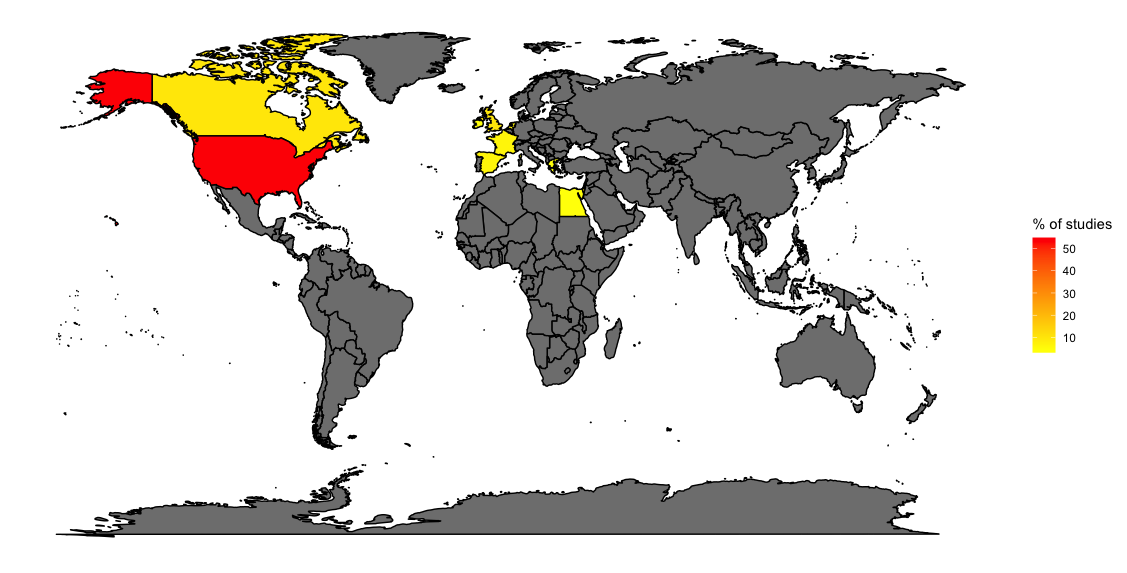
\includegraphics[width=\textwidth]{figures/KaelanandParafitaCouto-img002.png}
\caption{Percentage of studies on code-switching in neurodevelopmental conditions per country.}
\label{fig:kascelan:2}
\end{figure}

Considering the language combinations of neurodivergent participants, more than a third of the studies included English-Spanish bilinguals (n = 12), while 7 studies included a mix of participants speaking English and another language (Arabic, Armenian, Bangala, Danish, French, Gujarati, Hebrew, Hindi, Italian, Kachhi, Lithuanian, Mandarin, Polish, Portuguese, Punjabi, Russian, Spanish, Turkish, Urdu, Welsh). The following language combinations were each represented in two studies: Hebrew-English, English-Mandarin, Catalan-Spanish, Dutch-Turkish. Finally, there was 1 study focusing on each of the following language combinations: English-Irish, English-Mirpuri-Urdu, Hebrew-English-Hungarian, French and another language (English, Gujarati, Hindi, Marathi, Punjabi, Spanish). Looking at these findings, all but 4 studies (\citealt{Aguilar-MediavillaEtAl2024, BlomEtAl2024, Sanz-TorrentEtAl2007, SnijdersEtAl2025}) focused on participants speaking English in combination with another language.

The majority of studies (23/31) were conducted with children, while only 2 focused on adults and 2 included data from both children and adults. Data about age was missing or irrelevant in 4 studies. As shown in \figref{fig:kascelan:3}, most studies have been conducted with pre-school and early years school children. Gender or sex were explicitly labelled in 12 studies, only 1 of which (\citealt{AnguloJimenez2020}) inquired about both sex and gender. In the remaining 19 studies, the distinction was not explicitly mentioned, and 5 of these studies included no data on neurodivergent participants’ gender/sex. For the purposes of this review’s summary, all the binary sex/gender data is collated into male and female. Across the 31 studies, there were 199 male and 68 female neurodivergent participants. Two studies did not provide gender/sex breakdown of participants within the neurodivergent group; therefore, these participants (23 neurodivergent children in \citealt{KingEtAl2021}, and 13 neurodivergent children in \citealt{SoesmanEtAl2022}) are not included in our count.

The final demographic variable which we summarise is the socioeconomic status (SES) of participants. The breakdown across the studies was as follows: 7 studies included participants with low SES, 1 with medium SES, 5 with high SES, 3 with mixed SES, and 15 with no data on SES. Despite the authors’ consensus in coding the SES data, some of our decisions in coding might have misrepresented the SES status of the participants. For instance, if a study included a mean/median value of the SES status and a large range of scores without a clear indication of how the majority of the sample could be characterised, we labelled this as mixed SES (e.g., in the study by \citealt{SnijdersEtAl2025}). This however obscures the accurate representation of the sample. Furthermore, if the education of parents was the only SES indicator and the parents had a university degree of any level, we would code this as high SES (e.g., the study by \citealt{Yu2016}). Nevertheless, this approach is not necessarily an accurate representation, since families with a university degree do not necessarily have a high annual income.

As expected, SES was operationalised differently across the studies, thus making the task of data comparability quite challenging. About 42\% of the studies included education as an SES estimate (n = 13). Other indicators included: annual income (n = 3), occupation (n = 3), free/reduced lunch (n = 3), employment (n = 1), class indication (n = 1), low-high label (n = 1), missing data (n = 15). The raw numbers do not add up to the total number of papers included in this review (n = 31), as some of them included more than one SES indicator. A general summary of all the demographic variables can be found in \figref{fig:kascelan:3}.

\begin{figure}
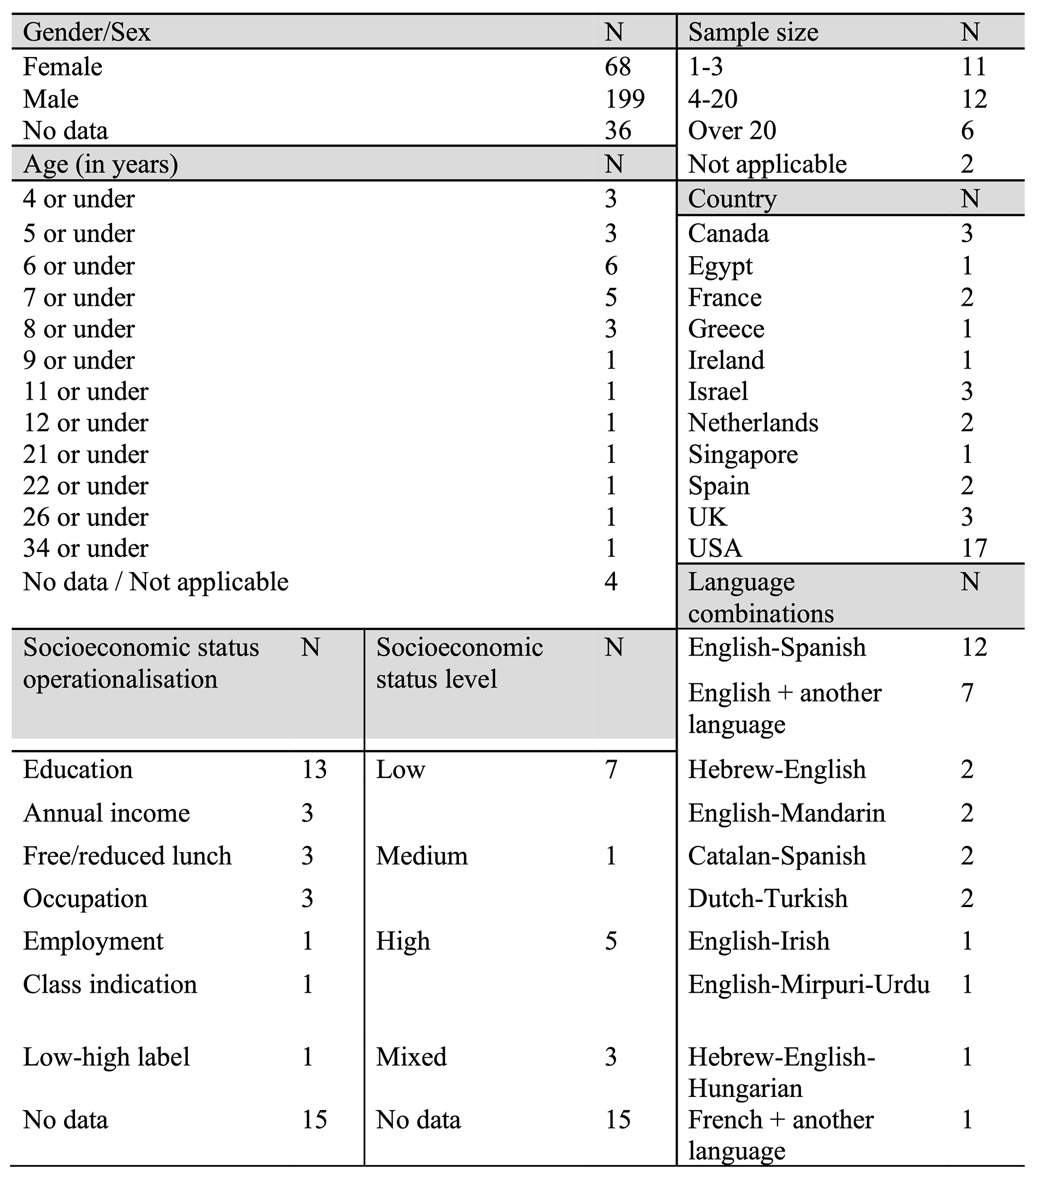
\includegraphics[width=\textwidth]{figures/KaelanandParafitaCouto-img003.jpg}
\caption{Demographic data of neurodivergent participants.}
\label{fig:kascelan:3}
\end{figure}

\subsection{Characteristics of neurodivergent code-switching and comparison groups}

One of the main goals of this review was to outline characteristics and any possible differences in code-switching practices (e.g., frequencies of code-switching, types of code-switching, etc.) of neurodivergent individuals in comparison to neurotypical code-switching. Of the 31 papers, 14 included a comparison group / individuals, 16 included no comparison group/individuals, and in the case of 1 study, comparison was not applicable as it explored professionals’ perceptions of language impairments in bilinguals (\citealt{O’TooleHickey2013}). 4 of the 16 studies which included no comparison groups/individuals compared the code-switching patterns of their neurodivergent participants to existing literature on neurotypical code-switching. This data is summarised in \tabref{tab:kascelan:3}.

\begin{table}
\footnotesize
\begin{tabularx}{\textwidth}{Q@{}Y@{~}Y@{~}Y@{~}Y}
\lsptoprule
Comparison of neurodivergent code-switching to neurotypical patterns & Studies with comparison groups{\slash}individuals\newline  (n = 14) & {Studies with no comparison groups{\slash}individuals\newline  (n = 16)} & Studies in which comparison was not applicable (n~=~1) & Total number per difference category\\
\midrule
Not different & 2 & 3 & 0 & 5\\
\tablevspace
Predominantly not different & 3 & 1 & 0 & 4\\
\tablevspace
Both different and similar & 3 & 0 & 0 & 3\\
\tablevspace
Predominantly different & 2 & 0 & 0 & 2\\
\tablevspace
Different & 3 & 0 & 0 & 3\\
\tablevspace
Inconclusive & 1 & 0 & 0 & 1\\
\tablevspace
Not applicable & 0 & 12 & 1 & 13\\
\lspbottomrule
\end{tabularx}
\caption{Comparison of neurodivergent to neurotypical code-switching (data represents number of studies).}
\label{tab:kascelan:3}
\end{table}

Considering the different methodological approaches used across the studies as well as different research aims, direct comparability of findings poses a significant challenge. Below we summarise the findings in four categories:
(1) studies that identified no or predominantly no differences between neurodivergent and neurotypical code-switching (n = 9),
(2) studies that identified different or predominantly different patterns of code-switching by neurodivergent individuals (n = 5),
(3) studies which identified both differences and similarities between the neurodivergent and neurotypical groups (n = 3), and
(4) studies with inconclusive results (n = 1).

The 9 studies which included no (or predominantly no) differences in code-switching between neurodivergent and neurotypical participants included a variety of tasks/approaches. Examples of no differences  include the following:
(a) no differences in the frequency of code-switching on language assessments, on a story (re)telling task, on a narrative elicitation task, or in spontaneous speech / a guided conversation (\citealt{Aguilar-MediavillaEtAl2024, Gutiérrez-ClellenEtAl2009, KapantzoglouEtAl2021, Pert2007, Ponce-Lawler2017, Sanz-TorrentEtAl2007})
(b) no differences in the types of switches, such as the part of speech that is being code-switched, the use of participant- and discourse-related insertions and alternations, or the types of switches used for specific communicative/pragmatic purposes  (\citealt{AnguloJimenez2020, Gutiérrez-ClellenEtAl2009, Ponce-Lawler2017, Yu2016})
(c) no differences in terms of abiding to the Matrix Language Framework constraints in children with SLI \citep{Gutiérrez-ClellenEtAl2009};
(d) no differences in gender agreement strategies in an acceptability judgement and a sentence completion task by an adult with Prader-Willi syndrome (\citealt{LicerasGarcia-Alcaraz2019}); (e) no differences in the language of insertions, production of words in the phonology of the other language, grammatical violations, and regularisation errors by children with SLI \citep{Sanz-TorrentEtAl2007}. In the four studies which identified predominantly no differences between neurodivergent and neurotypical children, minor differences that were identified included the following:
(a) children with SLI producing more verbs in the other language and fewer nouns than the age-matched comparison group \citep{Sanz-TorrentEtAl2007};
(b) on a story retell task children with DLD showed a higher use of alternations than their age-matched comparison group at age 8, but this difference disappeared at age 12 \citep{Aguilar-MediavillaEtAl2024};
(c) a child with autism did not code-switch in cases of direct/indirect quotations or to achieve narrative frame breaks \citep{Yu2016};
(d) children with SLI omitted or made errors in late system morphemes on verbs \citep{Pert2007}.

There were 5 studies which identified different patterns of neurodivergent code-switching in comparison to neurotypical expectations. \citet{Iluz-CohenWalters2012} identified that in narrative elicitation and story retell tasks children with language impairment code-switched more than neurotypical children both overall and in longer segments of speech. They further identified that unlike neurotypical children, children with language impairment code-switched somewhat more to their first language. On a sentence repetition task using monolingual and code-switched sentences, \citet{SoesmanEtAl2022} identified that on English stimuli, children with DLD produced more non-target switches than neurotypical children (non-target switches were instances when a participant produces a code-switch in a sentence repetition task for an item that was originally not code-switched). Furthermore, while the neurotypical children produced more non-target code-switches in Hebrew than in English stimuli, in the DLD group, there were no differences between languages. In a repeated word association task, \citet{ShengEtAl2012} identified that children with language impairment code-switched more from English to Spanish than from Spanish to English, while the neurotypical group demonstrated the opposite pattern. A study by \citet{CohenEtAl2025} compared spontaneous speech of a child with autism to that of his sister and parents. While they identified different frequencies of code-switching between family members during various activities and for specific purposes, they demonstrated how integral code-switching can be in multilingual families. Finally, \citet{BlomEtAl2024} identified that children with DLD mixed more often in the home language setting than the neurotypical children. Specifically, children with DLD tend to respond in the societal language more than neurotypical children when they are spoken to in the home language. Additionally, societal language proficiency had a stronger impact on mixing by children with DLD than by the neurotypical children. However, \citet{BlomEtAl2024} indicated that these differences diminished over time. We note that of these 5 studies which identified differences in neurodivergent code-switching in comparison to neurotypical patterns, only one was based on the analysis of spontaneous speech and it included a case study of an autistic child \citep{CohenEtAl2025}, while another study combined spontaneous speech data with semi-experimental data in their analysis \citep{BlomEtAl2024}. We address this point in light of implications for practitioners in the discussion section below.

As indicated in \tabref{tab:kascelan:3}, 3 studies identified both differences and similarities between neurotypical and neurodivergent code-switching. In terms of the identified differences, \citet{GrossKaushanskaya2022} found that on a scripted confederate dialogue task, children with DLD were more likely than neurotypical children to produce a response entirely in English when interacting with a monolingual Spanish speaker, even when their proficiency in both languages is taken into account. However, as noted by \citet{GrossKaushanskaya2022}, cognitive control also played a role in these types of switches and a larger sample would be required to investigate relevant interactions between different factors relevant for children’s code-switching practices. In \citet{SnijdersEtAl2025}, on a cued picture naming task, children with DLD made more errors (e.g., cross-language errors, wrong-word errors, and ‘I don’t know’ responses) and had longer reaction times than neurotypical participants. In \citet{GrossCastilla-Earls2023}, in the narrative samples, children with DLD engaged more in between-utterance code-switching than the neurotypical children. Furthermore, Spanish proficiency had a larger negative association with between-utterance switches in the sample of children with DLD. Some qualitative differences between the groups were also identified in terms of types of insertions. We note that these three studies used experimental and/or semi-experimental paradigms, which we address in the discussion section.

Finally, a study by \citet{KingEtAl2021} produced inconclusive results. Specifically, on a cued language switching task on most trials, children with language impairment had longer reaction times than children without language impairment. However, as the authors acknowledge, the fact that children with language impairment were significantly younger than neurotypical subjects and that this difference was not accounted for in the analyses suggests that the findings should be interpreted with caution.

\subsection{Professional advice and attitudes to code-switching}

The majority of studies reviewed here did not explicitly inquire about attitudes towards code-switching and professional advice received about the language mixing practices. Specifically, 26/31 studies included no data on professional advice on code-switching, 4 studies included negative advice and only 1 study included both positive and negative advice. Examples of negative advice were as follows:

\begin{quote}
Parents were also told that they were “creating chaos” in their child’s mind by switching between languages and exposing their child to various words. The teachers and therapists then went on to issue further warnings, such as “your child will become terribly confused,” or “become more lost.” This advice was given to families despite the reality that members of the families often spoke no English and would be unable to converse with the children if language choice was restricted. \citep[195]{Jegatheesan2011}\footnote{We note that in some studies, such as in \citet{Jegatheesan2011}, multilingual practice seems to be the norm in the studied families and a practice that they do not want to abandon despite the advice by professionals to stick only to the societal language.}
\end{quote}

\begin{quote}
Five of the parents believed that code-switching would cause confusion. For example, Jin said, “In the last 6 months, I’ve tried to speak to Henry as much as possible in English. I would try to speak just in English because people told me not to switch back and forth.” [...] Many of the professionals they encountered, however, appeared to be misinformed about bilingualism and its relationship to the development and learning of children with ASD. Their advice to parents often perpetuated deficit views of bilingualism, including notions that learning two languages would cause semilingualism and delay, that code-switching caused confusion, or that the use of home languages interfered with the learning of English. \citep[18-21]{Yu2013}
\end{quote}

\begin{quote}
[Jason's m]other: Learning two totally different languages at the same time and understand them properly and use them properly at the same time, she [the clinician] mentioned about that would be extremely difficult with the kids who have speech problem. \citep[1231]{Kremer-Sadlik2005}
\end{quote}

\begin{quote}
[O]ne mother (Arabic-speaking father and grandparents) remembered, “I really felt that we were to blame [for his speech delay]. All that switching back and forth caused the problem, not being consistent, and it was all our fault... that we really confused him. I believed he had a language processing disorder, and I believe we hurt him doing that, all that switching.”  (\citealt{YGarciaEtAl2012}: 12)
\end{quote}

Only 1 study (\citealt{HowardEtAl2021}) reported both positive and negative advice on code-switching.

\begin{description}
\item[Negative:]~\noindent

\begin{quote}
We were advised to stick to one language because sometimes it can be very confusing jumping from one language to another, and just to keep that consistency as well. (Nabani). […] Nabani intimates that she agrees with the advice. (\citealt{HowardEtAl2021}: 185)
\end{quote}

\item[Positive:]~\noindent

\begin{quote}
Eleanora describes this process: ‘we did ask the health visitor when he was little and he just said, “No speak both languages and he’ll be fine”, and that’s what we did and his first words were a mixture, some in English, some in Italian.’ (\citealt{HowardEtAl2021}: 185)
\end{quote}
\end{description}

Considering attitudes to code-switching, 22/31 studies included no data on this particular matter. Of the remaining 9 studies, negative attitudes were present in 5 of them (\citealt{HowardEtAl2021,Kay-RainingBirdEtAl2012,O’TooleHickey2013,YGarciaEtAl2012,Yu2013}), positive attitudes in 1 of them (\citealt{OudetEtAl2022}), and both positive and negative attitudes in 3 of them (\citealt{HowardEtAl2021,Kremer-Sadlik2005,WhartonEtAl2000}). An example of each is offered below.

\begin{description}
\item[Positive:]~\noindent

\begin{quote}
The ability to switch between languages in conversation was a welcome development for parents who were concerned about their choice to use their respective L1s with their children. [...] ClaraF2 commented [that] her son’s communication progress may have come about through natural developmental maturity. She also spoke about increased time at home during lockdown with both parents speaking their respective L1s in conversation as leading to her son’s expressive code-switching. (\citealt{OudetEtAl2022}: 8)
\end{quote}

\item[Negative:]~\noindent

\begin{quote}
[T]he therapists appeared cognisant of [the] threat [of code-switching in case of endangered languages such as Irish] in noting that the level of code-switching in the bilingual children with SLI was higher than expected. SLT 4: I have come across children who would use a lot more loan words than you would expect them to, so sticking -áil [Irish progressive marker] onto the end of English verbs, that kind of thing.  (\citealt{O’TooleHickey2013}: 102)
\end{quote}

\item[Both:]~\noindent

\begin{quote}
Roberta described each language as a ‘whole universe’ and suggested that code-switching may increase her child’s cognitive flexibility: One of the issues with autistic kids is, you know, that they can find it difficult to be flexible in situations, so the fact that he has to switch codes, so with the codes comes a whole universe almost, I think that actually is a good way of practising, you know, flexibility. (\citealt{HowardEtAl2021}: 184)
\end{quote}

\begin{quote}
Anna suggested that the increased challenge of switching between languages may encourage her son Dean to ‘keep his mind busy’ and avoid distraction. (\citealt{HowardEtAl2021}: 184)
\end{quote}

\begin{quote}
Conversely, some parents felt that the severity of their own child’s autistic symptoms -- that is the extent of their communicative difficulties -- rendered bilingualism unfeasible. After seeing her son distressed by her code-switching, Hira opted for a monolingual approach: Slowly I started working with him at mix-matching and he used to cry and then I said, “it’s fine” and I used to let him cry. “OK, you’re crying, it’s fine”... and we decided just one language.  (\citealt{HowardEtAl2021}: 186)
\end{quote}
\end{description}

We return to addressing the low frequency of work on this topic and predominantly negative advice and attitudes towards code-switching in the discussion section.

\section{Discussion}

This scoping review aimed to summarise the academic literature on code-switching in neurodevelopmental conditions. We now turn to discussing the findings of the review aims and drawing implications for researchers, practitioners, and multilingual families. Throughout the discussion, we also acknowledge limitations of the present review.

\subsection{Bias in focus}

We found that the most frequently studied neurodevelopmental conditions in relation to code-switching are language impairment / DLD and autism. Code-switching is linked to certain cognitive and communicative skills, which from a medical model perspective, can be impaired or affected in DLD and autism. This perspective therefore may explain why DLD and autism have been the most frequently explored conditions in relation to code-switching. As reported above, the increased presence of studies on autism is also linked to the first author’s familiarity with the autism and bilingualism literature. Nevertheless, even if we excluded the studies on autism and code-switching which were identified through other methods rather than through database search, autism would still represent one of the most commonly featured conditions in this review. A recent review on multilingualism in neurodevelopmental conditions similarly demonstrated that autism is often explored in relation to exposure to multiple languages \citep{UljarevićEtAl2016}. Moreover, \citet{PrévostTuller2021} identified a steady interest in the topic over the past few years. Therefore, while our own familiarity with the literature on autism and bilingualism affected the breakdown of identified papers in \tabref{tab:kascelan:2}, it is safe to say that autism is often more frequently studied in multilingual populations in comparison to many other neurodevelopmental conditions. With these findings in mind, there is a need for exploration of code-switching practices in conditions beyond language impairment and autism.

Despite identifying 31 studies on code-switching in neurodevelopmental conditions, only 58\% of them had code-switching as the main focus. Of 13 studies which explored code-switching sporadically, only 1 was identified via the database search. This illustrates the importance of going beyond the database search when conducting scoping reviews, as some of the research aims targeted in this review can be addressed only peripherally in certain studies and therefore easily missed out via the database search.

\subsection{Demographic (under)representation}

There is a striking similarity between the investigation of code-switching in neurodevelopmental conditions and general explorations of bilingualism in neurodivergent individuals. Specifically, the topic has been explored primarily in Western countries and in Indo-European languages. In this review, most of the participants resided in North America or in Western Europe, and all but 4 studies included (at least some) bilinguals speaking English in combination with other languages. This finding is partially biased due to the authors’ inclusion of literature published in languages that they could understand (English, Galician, Italian, Serbo-Croatian, Spanish). Nevertheless, this finding is particularly concerning as most regions of the world in which multilingualism happens to be frequent and/or code-switching happens to be the norm of communication are not represented in the research with neurodivergent individuals published so far.\footnote{Examples of code-switching practices of such communities have been described in the work by authors such as \citet{BalamDePradaPérez2016} in Belize, \citet{Aboh2020} in Sub-Saharan Africa, \citet{Lipski2017} in Ecuador, among many others.}

While for the purposes of summarising the data related to sex and gender we classified all participants under the labels male and female, we find that across the studies there is no unanimous way of reporting on gender and sex, which leads to lack of clarity in describing the demographic information. Specifically, 16\% of studies did not provide information on gender or sex, while only about 39\% of studies referred to gender or sex explicitly. Importantly, 45\% of studies did not explicitly mention whether data was collected on gender or on sex. Some similar findings have been identified across other reviews related to neurodivergent individuals. For instance, \citet{GirolamoEtAl2023studies} found that among the studies on language impairment in autistic school-aged children which reported information on gender/sex, 41\% did not specify whether they reported gender or sex data. This calls for more clarity in reporting practices in order to represent the identity of participants more accurately, as well as allow for precise summaries in studies that review the literature on neurodivergent populations.

Looking at the age of participants whose code-switching practices have been explored, apart from noting that the majority of studies (74\%) have been conducted with children (i.e., in individuals under 18 years of age), a striking finding is that the studies related to children included only younger participants. Specifically, all studies focusing only on children had participants aged 12 or under. This mirrors the findings by \citet{PrévostTuller2021}, who identified that explorations of bilingualism and autism are severely underrepresented among teenagers. Our findings extend this point to other neurodevelopmental conditions as well as to adult neurodivergent bilinguals, who are also underrepresented in our corpus of studies. These results are likely driven by the assumptions that code-switching might cause confusion in neurodivergent children as they develop -- consequently, the focus of most studies remains on younger children and their language development. However, considering that code-switching is often a community norm for many multilinguals across their lifespan (e.g., see \citealt{ParafitaBalamnodate}), more work is required across age groups to understand the dynamic nature of neurodivergent bilingualism both from the personal and the linguistic perspective – for instance, what role does code-switching play across the lifespan of neurodivergent bilinguals, how does it link to their identity, and do linguistic changes in code-switching patterns emerge at different ages or across various generations of speakers (for some work on this topic in neurotypical bilinguals, see for instance  \citealt{GeorgalidouEtAl2010})? Importantly, grasping the nature of code-switching practices among older children and in adults can also inform practitioners more accurately in terms of life outcomes of neurodivergent bilinguals related to their linguistic identity and characteristics.

The final variable which we address in terms of representation across the reviewed studies includes SES. We acknowledge the limitation of our approach in classifying studies on a scale from low to high SES based on certain estimates used across research. For instance, to enable the summary of the data we made the decisions such as classifying studies where the caregivers have predominantly any higher education degree as high SES. However, while holding a university degree does not necessarily imply high SES, in multilingual contexts linked to migration the connection between a university degree and high SES is even weaker. Recent data from the UK context show that 20\% of UK born workers are overqualified for what is labelled as low or medium-low skilled jobs (\citealt{Fernandez-ReinoBrindle2024}). This percentage increases to 26\% for all foreign-born workers, and to 27\%-29\% for workers from Central and South America, European Union (EU) as a whole, Middle East and North Africa and Central Asia, and Sub-Saharan Africa. The increase goes to 39\%-44\% when it comes to workers from EU-2 countries, Pakistan and other South Asian countries, and EU-8 countries (\citealt{Fernandez-ReinoBrindle2024}).\footnote{EU-2 countries include Romania and Bulgaria, while EU-8 countries include Poland, Lithuania, Czech Republic, Hungary, Slovakia, Slovenia, Estonia, and Latvia.} Among the studies in this review, 13 studies (42\%) included education as an indicator of SES, 7 of them in combination with other estimates. Considering the data from \citet{Fernandez-ReinoBrindle2024}, research on multilingualism should avoid relying solely on education as an SES estimate. Implementing the approach by \citet{GirolamoEtAl2023studies}, who ascribed higher quality to studies which reported SES using more than one indicator, we find that only 8/31 studies (26\%) did so in the present review (\citealt{AnguloJimenez2020, CohenEtAl2025, GrossCastilla-Earls2023, Gutiérrez-ClellenEtAl2009, KapantzoglouEtAl2021, ShengEtAl2012, Yu2013}). While it remains challenging to outline recommendations on which SES estimates are more adequate for specific contexts, moving beyond a single variable as an SES estimate needs to be prioritised in future research for a more accurate representation of investigated populations.

\subsection{Characteristics of neurodivergent code-switching}

We now turn to discussing one of the main aims of this scoping review -- is code-switching by neurodivergent individuals different from that of neurotypical individuals, and if so, what implications does this have? We interpret these findings in relation to the methodological characteristics of the papers reviewed, as well as the attitudes identified and professional advice on code-switching in neurodivergent contexts. Of the 18 studies which included some sort of comparison in code-switching between neurodivergent and neurotypical individuals, 9 (50\%) identified no or predominantly no differences, 5 (28\%) identified (predominantly) different code-switching patterns, 3 (17\%) included both similarities and differences, and 1 (6\%) produced inconclusive results. As noted in the results section, identified differences in code-switching patterns do not necessarily imply a deficit. Importantly, there is a need to contextualise these findings in terms of the existing stigma towards code-switching, especially in a neurodivergent context. In particular, most studies to date identified a negative attitude towards code-switching and negative advice received from professionals, such as educators or speech and language therapists. Considering that such stigmatisation of code-switching impacts communicative practices of multilingual families, it likely affects how neurodivergent individuals code-switch. Specifically, preventing exposure to the code-switching community norms (in terms of frequency, types of code-switches, etc.) could lead to different patterns in neurodivergent code-switching. Consequently, any differences in code-switching identified across studies in this review could be related to changes in family communicative practices based on code-switching stigmatisation or pathologisation. This further reinforces a need for explorations of neurodivergent code-switching in communities in which multilingualism is the norm and in which stigma about code-switching is non-existent or lower than in the West European and North American contexts, which were overrepresented in this review.

We note that our conservative approach to data extraction on attitudes and advice on code-switching likely impacted the representation of negative views and recommendations. Specifically, we counted instances of attitudes and professional advice only when language mixing was explicitly mentioned. However, negative advice regarding bilingualism in general (e.g., speaking to the child only in the societal language and dropping the home languages) is commonly identified in studies on neurodivergent bilinguals \citep{UljarevićEtAl2016}. Considering this, in the present review we focused only on advice and attitudes towards language mixing explicitly. Nevertheless, we acknowledge that professional advice to use only the societal language with the child inevitably implies avoiding code-switching. This suggests that negative attitudes/advice on code-switching are likely more prevalent than what we report. Consequently, any observed differences in neurodivergent code-switching need to be interpreted cautiously. Our conclusion based on the studies in this review is that observed differences in neurodivergent code-switching do not imply a deficit or a reason for concern.

How generalisable these findings are also depends on methodological characteristics of the observed studies. Taking into account the ways in which code-switching has been explored across the studies, only 19\% of studies used spontaneous speech data and an additional 13\% of studies used a combination of spontaneous speech and a semi-experimental task. While semi-experimental data can be reflective of code-switching community norms, spontaneous speech data represents the most accurate description of community practices and it facilitates the understanding of data obtained through (semi)experimental approaches (e.g.,  \citealt{vanOschEtAl2023, ParafitaCoutoEtAl2024, Vaughan-EvansEtAl2020}). In the present review, 19\% of studies used a purely experimental approach in exploring code-switching in neurodivergent bilinguals. Considering the impact that this research can have on the decisions that multilingual families make about language practices with their neurodivergent family members, we invite researchers to be cautious in their study designs and interpretations of their findings. For instance, using sentence repetition tasks or repeated word association tasks (such as in \citealt{SoesmanEtAl2022} or in \citealt{ShengEtAl2012}), cued picture selection or naming tasks (as in \citealt{KingEtAl2021} or \citealt{SnijdersEtAl2025}, acceptability judgement and sentence completion tasks (such as in \citealt{LicerasGarcia-Alcaraz2019}) does not necessarily reflect ecologically valid code-switching practices. In fact, some of these tasks (e.g., the cued picture naming task in \citealt{SnijdersEtAl2025}) are better described as verbal cognitive rather than linguistic tasks. Therefore, identifying differences between neurodivergent and neurotypical bilinguals by using solely experimental paradigms could lead to increased concerns about language mixing practices of neurodivergent bilinguals, while in fact such tasks do not necessarily reflect the true nature of their bilingual competencies or the role that code-switching can play in their communicative practices or in creating bonds with their families or communities.

A part of the problem is related to the terminology used when exploring code-switching. Due to the lack of consensus on code-switching terminology in the field, and for the purposes of scoping any relevant work on this topic, in this review we used terms such as code-switching, language mixing, code mixing (and others) interchangeably. While we defined code-switching in the introductory section, it is clear that the work reviewed in this paper goes beyond that phenomenon and in some cases (e.g., \citealt{SnijdersEtAl2025}), it includes work on cognitive skills rather than what we consider code-switching. While the debates on differences and similarities between the terms used and phenomena will inevitably carry on and change over time, we invite researchers to continue (and in cases when they have not done so, start) describing in detail the phenomenon under investigation to enable accurate comparability in research. In addition, we note that the lack of consensus on code-switching definitions seems to exist in general (e.g., \citealt{GullbergEtAl2009}) and not only when exploring code-switching in individuals with neurodevelopmental conditions. While the comparison of code-switching definitions across the studies was beyond the scope of this review (see the aims outlined in the pre-registered protocol: \citealt{KascelanParafitaCouto2022}), we encourage researchers to pursue this research question in future reviews on the topic. Importantly, we also invite researchers to make an additional effort to communicate or clarify their work to relevant stakeholders (e.g., multilingual families, neurodivergent individuals, speech and language therapists, teachers, medical experts) in such a way that prevents findings on related but different phenomena from being misused in advising multilingual families of neurodivergent individuals to drop their home languages or ban/restrict code-switching practices in their interactions.

\subsection{Generalisability of findings}

We now turn to a common trend of small samples in research on neurodivergent bilinguals and the implications for finding generalisability. In addition to the fact that code-switching in neurodivergent bilinguals is underexplored, we found that only 6 studies included samples of more than 20 participants. This corroborates a recent review on bilingualism and autism research, which identified small sample sizes across quantitative studies (\citealt{PrévostTuller2021}). In light of these circumstances, there is a question of how generalisable quantitative studies with smaller samples are. As suggested by \citet{GirolamoEtAl2023studies}, working with small and heterogeneous groups (in this case heterogeneous both in terms of neurodivergent and bi{\slash}multilingual status, as well as potentially racial, gender/sex, or socioeconomic characteristics) requires selecting analytic approaches more adequate for such samples (e.g., Bayesian approaches). We also note that the application of qualitative methods could further illuminate our understanding of neurodivergent bi/multilinguals’ lived experiences in ways not necessarily captured with purely quantitative perspectives (e.g., see  \citealt{HowardEtAl2019} on using Interpretative Phenomenological Analysis in autism research). The combination of quantitative and qualitative approaches is particularly important to consider when exploring community norms of code-switching practices. Specifically, as variation in code-switching community norms can be expected (see \citealt{Deuchar2020,ParafitaBalamnodate}), relying on benefits of mixed methods approaches can help us understand how the heterogeneous nature of neurodivergent bilingualism interacts with established community norms.

The issue of smaller samples and lack of generalisability could somewhat be mitigated following suggestions by \citet{PrévostTuller2021} on large-scale inter-lab collaborations. In code-switching research with neurodivergent bilinguals, this could include designing and sharing a protocol for spontaneous speech studies, which would be used across various communities/locations. Apart from a general agreement to collect spontaneous speech data, the protocol could include a list of tools to use for obtaining relevant background information about the participants’ conditions and their bi/multilingual experiences. Taking into account the diversity and lack of equivalency between the questionnaires used to document bi/multilingualism (see \citealt{KascelanEtAl2022} for questionnaires used with children and \citealt{DassEtAl2024} for questionnaires used with adults), it would be important to use a set of shared tools across labs to ensure data comparability. Projects such as Many Babies\footnote{See \url{https://manybabies.org/index}.}  represent a useful example of how such large-scale inter-lab collaborations could be established and navigated.

Inter-lab collaborations would likely contribute to more generalisability through the creation of aggregated datasets, provided there is full data availability. However, access to existing corpora of spontaneous speech of bi/multilinguals is a commonly documented issue in code-switching research even in neurotypical samples (\citealt{Deuchar2020,ParafitaCoutoetal2023,ParafitaCoutoEtAlinpress}). We strongly agree with the call for making (anonymised) corpora of spontaneous speech fully available. However, care must be taken when making the data accessible to the public particularly when working with vulnerable groups (e.g., neurodivergent individuals, minoritised speakers). Neurotypical researchers are automatically outsiders to neurodivergent communities that they work with. This makes it even more important to approach such projects in a participatory way through the creation of trust and community partnerships. As outlined in  \citet{GirolamoEtAl2023community}, a part of this process includes dynamic and interactive informed consent and assent, which as an iterative process would give participants a higher level of control of their own data, while ultimately also making the datasets available to the public whenever possible. Taking such a community-based approach takes years to develop (e.g., see \citealt{GirolamoEtAl2023community} for an example of such a project including a 7-year timeline); nevertheless, a community-based approach enables removal of barriers in recruitment of neurodivergent bilinguals, it helps co-construct accurate narratives about their participation and languaging, and it contributes to responsible data sharing as well as to research transparency. This approach reinforces the importance of slow science for responsible and high-quality research (\citealt{Fletcher-WatsonEtAl2019,GirolamoEtAl2023community}) and has implications for funding bodies which often fund only short-term projects. Importantly, slow science requires opposing policies of the neoliberal university and the constant requirement for researchers to compete for rankings and publish at a fast pace. Without a culture in which researchers are given time and resources required to conduct studies that include community-based approaches, the work with neurodivergent bilinguals will likely continue facing similar limitations as it has had in the up-to-date research presented in this review and elsewhere (see \citealt{PrévostTuller2021}).

\subsection{Implications for practitioners and multilingual families}

We now turn to the implications for practitioners (primarily speech and language therapists and educators working with neurodivergent individuals). Some of these points are also relevant to neurodivergent individuals and their families. Overall, the review indicates that code-switching does not pose a difficulty or threat for a neurodivergent individual’s development or language use. On the contrary, across several studies, neurodivergent individuals have used code-switching as a demonstration of their communicative competences (e.g., \citealt{AnguloJimenez2020,Ponce-Lawler2017,Yu2016}). Importantly, any observed differences in code-switching patterns between neurodivergent and neurotypical individuals need to be interpreted in light of contextual factors (i.e., predominantly negative attitudes and advice on code-switching) as these might affect the code-switching characteristics of neurodivergent individuals (e.g., the code-switching frequency, the types of code-switches, the contexts in which they code-switch). Additionally, individual variations in code-switching patterns can be expected among neurotypical individuals as well (e.g., \citealt{CohenEtAl2025}). Therefore, when variation in code-switching emerges among neurodivergent individuals, it should not be pathologised by default. Considering this, we advise practitioners not to discourage multilingual families from code-switching with their neurodivergent family members, especially when code-switching is a part of their family’s/community’s communicative practice. These recommendations are the extension to the emerging evidence in bilingualism literature, which suggests that being neurodivergent or having a neurodivergent family member should not imply opting for monolingualism (e.g., \citealt{DigardEtAl2023,PrévostTuller2021,UljarevićEtAl2016}). This is particularly important considering the evidence about the link between maintaining family multilingualism and family wellbeing \citep{MullerEtAl2020}.

Nevertheless, we also point practitioners to cases when neurodivergent individuals express negative attitudes to code-switching or to the use of / exposure to one of their languages. For instance, a case study of a child with stutter identified the child’s negative attitude towards using the home language \citep{Karniol1992}. As a part of evidence-based practice, it is critical that speech and language therapists consider the following three elements: their clinical expertise, the service user’s preferences and values, and scientific evidence (\citealt{HealthandCareProfessionsCouncil2023, Royalnd}). Therefore, when individuals show reluctance to use all of their languages (which likely includes avoiding code-switching), the healthcare professionals should not aim to enforce communicative practices not preferred by the service users. Instead, they should present the available evidence on multilingualism (which could address possible stigma associated with multilingualism and code-switching) so that neurodivergent individuals and their families can make informed decisions about their preferences.

The research on stigma towards code-switching and multilingualism in general requires further investigation. We suspect that identifying predominantly negative advice and attitudes on code-switching in this review is linked to the fact that most of the reviewed studies were conducted in countries with monolingualism-centric views. Apart from continuing the investigation of this topic in the communities included in this review, it is imperative to learn about the code-switching phenomenon (especially in relation to neurodivergent individuals) from underexplored parts of the world where multilingualism is the norm. We also invite researchers exploring this topic to make a clear distinction between attitudes/advice on multilingualism and attitudes/advice on code-switching. Specifically, while in some monolingualism-centric countries, attitudes on multilingualism might be improving (e.g., see \citealt{DigardEtAl2023}), the stigma on code-switching could still remain due to the pressure imposed by standard language ideologies and their prescriptivist, puristic and racialised views of communicative practices.

\section{Concluding remarks}

This scoping review outlines the existing findings on code-switching in bi{\slash}multilinguals with neurodevelopmental conditions. Generally, we do not identify evidence of harmful effects of code-switching for neurodivergent individuals. In light of this, we make recommendations for practitioners, especially speech and language therapists and educators working with neurodivergent individuals. We do however find that this topic remains severely underexplored and the existing evidence suffers from bias in focus (primarily on DLD and autism) and demographic underrepresentation (i.e., focus has been mostly on younger children, on specific geographic locations and language combinations). We further observe that the lack of terminological consensus on code-switching translates from research with neurotypical individuals onto the research with neurodivergent population. We invite researchers to consider how they communicate their findings (especially in relation to neurodivergent population) as some of the used experimental approaches explored related constructs to code-switching but not code-switching per se. Therefore, these findings should not be the core literature informing recommendations on code-switching practices in neurodivergent contexts. In light of these downsides, we discuss generalisability of existing findings and offer suggestions about methodological and practical issues in exploring this topic.

We would also like to highlight that while our key search terms included terminology related to code-blending for the purposes of including work from sign languages, we did not succeed in identifying any relevant work. Consequently, this review is focused on the spoken modality only, so we encourage researchers to pursue this topic taking into account multimodal perspectives. Finally, this review focused on neurodevelopmental conditions. Considering that bilingualism is often a lifelong and a dynamic experience, there is a need to explore code-switching practices in acquired conditions as well. Relevant discussions of code-switching in conditions such as aphasia can be found in \citet{Aboh2020}.

\section*{Supplementary materials}

The datafile can be accessed on the project's OSF page: \url{https://osf.io/4nwgd/}

% Note: The studies included in the scoping review are marked with an asterisk.

\sloppy\printbibliography[heading=subbibliography,notkeyword=this]
\end{document} 
